\documentclass[nobib]{tufte-handout}

%\\geometry{showframe}% for debugging purposes -- displays the margins

\newcommand{\bra}[1]{\left(#1\right)}
\usepackage{amssymb}
\usepackage{hyperref}
\usepackage[activate={true,nocompatibility},final,tracking=true,kerning=true,spacing=true,factor=1100,stretch=10,shrink=10]{microtype}
\usepackage{color}
\usepackage{steinmetz}
% Fixes captions and images being cut off
\usepackage{marginfix}
\usepackage{array}
\usepackage{tikz}
\usepackage{amsmath,amsthm}
\usetikzlibrary{shapes}
\usetikzlibrary{positioning}
\usepackage{listings}
\usepackage{caption}
\usepackage{circuitikz}
\DeclareCaptionFont{white}{\color{white}}
\DeclareCaptionFormat{listing}{\colorbox{gray}{\parbox{\textwidth}{#1#2#3}}}
\captionsetup[lstlisting]{format=listing,labelfont=white,textfont=white}

% Set up the images/graphics package
\usepackage{graphicx}
\setkeys{Gin}{width=\linewidth,totalheight=\textheight,keepaspectratio}
\graphicspath{{.}}

\title{Notes for ECE 20002 - Electrical Engineering Fundamentals II}
\author[Shubham Saluja Kumar Agarwal]{Shubham Saluja Kumar Agarwal}
\date{\today}  % if the \date{} command is left out, the current date will be used

% The following package makes prettier tables.  We're all about the bling!
\usepackage{booktabs}

% The units package provides nice, non-stacked fractions and better spacing
% for units.
\usepackage{units}

% The fancyvrb package lets us customize the formatting of verbatim
% environments.  We use a slightly smaller font.
\usepackage{fancyvrb}
\fvset{fontsize=\normalsize}

% Small sections of multiple columns
\usepackage{multicol}

% For finite state machines 
\usetikzlibrary{automata} % Import library for drawing automata
\usetikzlibrary{positioning} % ...positioning nodes
\usetikzlibrary{arrows} % ...customizing arrows
\tikzset{node distance=2.5cm, % Minimum distance between two nodes. Change if necessary.
    every state/.style={ % Sets the properties for each state
    semithick,
    fill=gray!10},
    initial text={}, % No label on start arrow
    double distance=2pt, % Adjust appearance of accept states
    every edge/.style={ % Sets the properties for each transition
    draw,
    ->,>=stealth', % Makes edges directed with bold arrowheads
    auto,
    semithick}}
\let\epsilon\varepsilon

% These commands are used to pretty-print LaTeX commands
\newcommand{\doccmd}[1]{\texttt{\textbackslash#1}}% command name -- adds backslash automatically
\newcommand{\docopt}[1]{\ensuremath{\langle}\textrm{\textit{#1}}\ensuremath{\rangle}}% optional command argument
\newcommand{\docarg}[1]{\textrm{\textit{#1}}}% (required) command argument
\newenvironment{docspec}{\begin{quote}\noindent}{\end{quote}}% command specification environment
\newcommand{\docenv}[1]{\textsf{#1}}% environment name
\newcommand{\docpkg}[1]{\texttt{#1}}% package name
\newcommand{\doccls}[1]{\texttt{#1}}% document class name
\newcommand{\docclsopt}[1]{\texttt{#1}}% document class option name

% Define a custom command for definitions and biconditional
\newcommand{\defn}[2]{\noindent\textbf{#1}:\ #2}
\let\biconditional\leftrightarrow

\begin{document}

\maketitle

\begin{abstract}
    These are lecture notes for spring 2024 ECE 20002 at Purdue. Modify, use, and distribute as you please.
\end{abstract}

\tableofcontents

\section{Course Introduction}

Continuation of Electrical Engineering Fundamentals I. The course addresses
mathematical and computational foundations of circuit analysis (differential
equations, Laplace Transform techniques) with a focus on application to linear
circuits having variable behavior as a function of frequency, with emphasis on
filtering. Variable frequency behavior is considered for applications of
electronic components through single-transistor and operational amplifiers. The
course ends with a consideration of how circuits behave and may be modeled for
analysis at high frequencies.\\~\\ Learning Objectives:
\begin{enumerate}
    \item Analyze 2nd order linear circuits with sources and/or passive elements
    \item Compute responses of linear circuits with and without initial conditions via
          one-sided Laplace transform techniques
    \item Compute responses to linear circuits using transfer function and convolution
          techniques
    \item Analyze and design transistor amplifiers at low, mid and high frequencies
\end{enumerate}

\pagebreak

\section{ECE 20001 Review}
Sinusoidal Signal (voltage and current) involve phasors, which bring complex
numbers to the forefront. When in Sinusoidal Steady State (SSS):\\
\begin{equation*}
    Z_R=R
\end{equation*}
\begin{equation*}
    Z_L=j\omega L
\end{equation*}
\begin{equation*}
    Z_C=\frac{1}{j\omega C}
\end{equation*}
This can in turn be represented as as the following function:\\
\begin{equation*}
    x(t)=K_0 cos(\omega t + \theta_0)
\end{equation*}
Which can be transformed into the following form:\\
\begin{align*}
    K_0 e^{j(\omega t + \theta_0)} & = K_0 e^{j \theta_0}                    \\
                                   & = K_0 (cos(\theta_0) + j sin(\theta_0)) \\
                                   & = K_0\phase{\theta_0}
\end{align*}
This can be represented as the following in the cartesian plane:\\
\begin{center}
    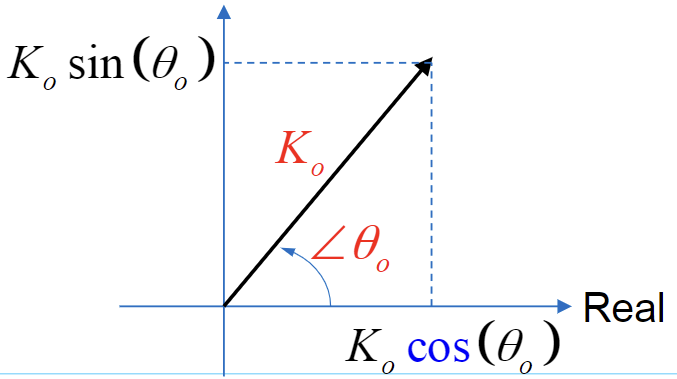
\includegraphics[width = 150px]{images/Screenshot 2024-01-08 155954.png}
\end{center}
Thus, these forms can be summed as following:\\
\begin{table}
    \centering
    \begin{tabular}{c|c}
        x(t)                                & $\mathbf{X}$ \\
        \hline
        $K cos(\omega t)$                   & K            \\
        $K sin(\omega t) = K cos(\omega t)$ & $-Kj$        \\
        $cos(\omega t) - sin(wt)$           & $1+j$        \\
        $a cos(\omega t) + b sin(\omega t)$ & $a-bj$
    \end{tabular}
\end{table}
This is especially useful for circuit analysis methods such as KCL and KVL.
The methods of conversion between polar and phasor are:\\
\begin{equation*}
    z=a+bj
\end{equation*}
\begin{equation*}
    z=\rho \phase{\theta}
\end{equation*}
\begin{equation*}
    \rho = |z| = \sqrt{a^2 + b^2}
\end{equation*}
\begin{equation*}
    \theta = \text{phase(}z\text{)}=tan^{-1}(\frac{b}{a})
\end{equation*}
These conversions and operations alongside KCL and KVL, can allow us to create a system of differential equations that will allow us to solve almost any circuit. However, we don't like ODEs, so we have developed methods to get around this.\\
We know that at SSS, the following equations are valid.
\begin{center}
    \begin{align*}
        V_R    & = RI_R                               \\
        V_L    & = j\omega LI_L                       \\
        V_C    & = \frac{1}{j \omega C}I_C            \\
        V_L(t) & = L\frac{di_L}{dt}        & \implies
        i_L(t) = i_L(0) + \frac{1}{L} \int v_L \,dt   \\
        i_C(t) & = C\frac{dV_C}{dt}        & \implies
        V_C(t) = V_C(0) + \frac{1}{C} \int i_C \,dt   \\
    \end{align*}
\end{center}
This can be used to solve most (to the knowledge of the student till this point) SSS circuits. Strategies have been developed to simplify these calculations. Some examples of this are current and voltage division, with the impedance $Z$ replacing the linear $R$. Strategies like these allow the resolution of circuits like these while avoiding higher order differential equations.\\
Example:
\begin{center}
    \begin{circuitikz}[american currents]
        \draw (0,0)
        to[I, l=$I$] (0,2)
        to [short, -*] (1,2)
        to [L, l=$L$] (1,0)
        to [short, -] (0,0);
        \draw (1,2)
        to [short, -*] (2,2)
        to [R, l=$R$] (2,0)
        to [short, *-*] (1,0);
        \draw (2,2)
        to [short, -] (2.5,2);
        \draw (2,0)
        to [short, -] (2.5,0);
    \end{circuitikz}
\end{center}
\begin{align*}
    I_R=\frac{Z_L}{Z_R+Z_L}*I=\frac{j \omega L}{R+j \omega L}*I \\
    I_L=\frac{Z_R}{Z_R+Z_L}*I=\frac{R}{R+j \omega L}*I
\end{align*}
If this circuit had an additional energy storing component, such as a capacitor
or an additional inductor, the complexity of current division does not increase
by a lot, but the differential equation would go from being a first-order differential
equation to a second-order differential equation. The complexity of this would be much
higher than that of the first-order differential equation, and would continue increasing
for each energy storing component that is added to the circuit.\\
Note: All of this is based on the assumption of \textbf{Sinusoidal Steady State}.
\\~\\
\begin{center}
    "We don't like differential equations." -Prof. Byunghoo Jung
\end{center}
\pagebreak
\section{Using Ordinary Differential Equations to solve RL and RC circuits}
This section will provide a brief explanation of nonhomogenous differential
equations and their applications to circuits (Completely ignoring the fact that
we in fact do not like them, as repeatedly stated in the previous section).
\subsection{Ordinary Differential Equations (ODE) Overview}
Differential equations rely a lot on two properties. The invariability of the
exponential function across derivatives, and the ability to express any
function in terms of the exponential function itself. That is,\\
\begin{equation*}
    e^t=\frac{d}{dt}e^t=\frac{d^2}{dt^2}e^t \cdots
\end{equation*}
Let us take the following differential equation as an example:
\begin{equation*}
    y(t)=6x(t)+3\frac{d}{dt}x(t)
\end{equation*}
Because of the beauty (invariability) of the exponential function, we assume $x_h(t)=Ae^{\lambda t}$, and try to solve the homogenous equation $0=6x(t)+3x'(t)$.
\begin{align*}
    0               & = 6x+3x'                                     \\
    0               & = 6Ae^{\lambda t} + 3A \lambda e^{\lambda t} \\
    0               & = 6+3\lambda                                 \\
    \lambda         & = -2                                         \\
    \implies x_h(t) & = e^{-2t}
\end{align*}
At this point, we will consider two different cases: $y(t) = 4e^{3t}$ and $y(t) = 3e^{-2t}$.
We will find the particular solution $x_p(t)$ for each of these cases, as they have different methods of resolution.
\begin{align*}
    4e^{3t}               & = 6x+3x'                                    \\
    \text{Assume } x_p(t) & = Be^{3t}                                   \\
    4e^{3t}               & = 6Be^{3t} + 9Be^{3t}                       \\
    4                     & = 15B                                       \\
    B                     & = \frac{15}{4}                              \\
    \implies x_p(t)       & = \frac{15}{4}e^{3t}                        \\
    \implies x(t)         & = x_h(t)+x_p(t)=Ae^{-2t}+\frac{15}{4}e^{3t}
\end{align*}
Let us assume $y(0) = 4$
\begin{align*}
    \implies 4    & = A + \frac{15}{4}                      \\
    \implies A    & = \frac{1}{4}                           \\
    \implies x(t) & = \frac{1}{4}e^{-2t}+\frac{15}{4}e^{3t}
\end{align*}
On the other hand, if $y(t) = 3e^{-2t}$, since $x_p(t)$ and $x_h(t)$ cannot have the same form, we will need to make a few changes:
\begin{align*}
    3e^{-2t}              & = 6x+3x'                              \\
    \text{Assume } x_p(t) & = Bte^{-2t}                           \\
    3e^{-2t}              & = 6Bte^{-2t} + 3Be^{-2t} - 6Bte^{-2t} \\
    \implies 3            & = 3B                                  \\
    \implies B            & =1                                    \\
    \implies x_p(t)       & = te^{-2t}
\end{align*}
Which can then be substituted into $x(t)$, allowing the differential equation to be fully solved by using the initial conditions.
\subsection{Using ODEs in circuits}
We will be solving the following two circuits (Note: you will never see
something like this with a current source instead, because it would be too
easy):
\begin{center}
    \begin{circuitikz}[american voltages]
        \draw (0,2)
        to[V, l=$V_{in}$] (0,0);
        \draw (0,2)
        to [R, l=$R$] (2,2)
        to [L, l=$L$] (2,0)
        to [short, -] (0,0);
    \end{circuitikz}
    \begin{circuitikz}[american voltages]
        \draw (0,2)
        to[V, l=$V_{in}$] (0,0);
        \draw (0,2)
        to [R, l=$R$] (2,2)
        to [C, l=$C$] (2,0)
        to [short, -] (0,0);
    \end{circuitikz}
\end{center}
In the inductor circuit, if $i_L(0)=0$, we know:
\begin{align*}
    v_L       & = L\frac{di_L(t)}{dt}                                  \\
    v_L(t)    & = v_{in}(t) + Ri_L(t)\text{ because of KVL}            \\
    v_{in}(t) & = L\frac{di_L(t)}{dt} + Ri_L(t)\text{ by substituting}
\end{align*}
By dividing the timeline into two sections, $(-\infty, 0) \text{ and } (0,\infty)$, and solving for the second one we can find our desired values for anytime in the future. However, for this to be a viable option, we need to solve for a continuous variable, which is $i$ for an inductor, and $v$ for a capacitor.\\
By solving this equation as shown previously, and looking for $i_L$, we will find that $\lambda = -\frac{R}{L}$ which is in fact the inverse of the time constant for an RL circuit.
Under the assumption of $V_{in}$ being a constant, the particular solution will in fact be $i_p(t)=\frac{V_{in}}{R}=i_L(\infty)$. This results in the familiar equation:
\begin{equation*}
    i_L(t) = i_L(\infty) + (i_L(t_0)-i_L(\infty))e^{-\frac{R}{L}(t-t_0)}
\end{equation*}
The same is done for the capacitor circuit, but this time looking for $v_C$, which ends up resulting in the once again familiar equation:
\begin{equation*}
    v_C(t) = v_C(\infty) + (v_C(t_0)-v_C(\infty))e^{-\frac{t-t_0}{RC}}
\end{equation*}
Note: energy storing components (L \& C) have memory but cannot consume power. R can consume power but has no memory.\\
Looking at this conceptually, the resistor is consuming energy at an exponential rate. This causes current, voltage, and all other signals to decay exponentially as well.\\
Since $P = I^2R = \frac{V^2}{R}$, it makes sense for the time constant to be $\tau = \frac{L}{R} = RC$, for each of them, as a larger capacitor or inductor would store more energy, and the proportionality of the R to the power and current or voltage respectively. That is, if R is larger, the power consumption is larger for an RL and smaller for an RC.\\
Note: the particular solution of the ODE is a scaled version of the input.\\
The homogenous solution will be the same for all inputs, and of the form $Ae^{\frac{-t}{\tau}}$.\\
The particular solution represents the behavior of the analyzed parameter when everything has settled down, or, at infinity.\\
Let us look at the particular resolution with a forcing equation of the form $v_{in}(t) = A\sin(\omega t)u(t)$.
\begin{align*}
    v_{C,p} & = \frac{Z_C}{Z_R+Z_C}V_{in}                              \\
            & = \frac{\frac{1}{j\omega C}}{R+\frac{1}{j\omega C}}(-Aj) \\
            & = \frac{1}{j\omega RC+1}(-Aj)
\end{align*}
Developing and simplifying that equation can lead to the form $A_1\cos(\omega t)+A_2\sin(\omega t)$.\\
These can then be substituted into the complete form, and, using the initial conditions, completely define the reactions.
We will now analyze the following circuits, which resemble the previous ones, but use voltage instead, and have the components in parallel instead of series.
\begin{center}
    \begin{circuitikz}[american voltages, american currents]
        \draw (0,0)
        to[I, l=$I_{in}$] (0,2);
        \draw (0,2)
        to [short, -] (1,2)
        to [R, l^=$R$] (1,0)
        to [short, -] (2,0)
        to [L, l_=$L$] (2,2);
        \draw (0,0) to [short, -] (1,0);
        \draw (1,2) to [short, -] (2,2);
    \end{circuitikz}
    \begin{circuitikz}[american voltages, american currents]
        \draw (0,0)
        to[I, l=$I_{in}$] (0,2);
        \draw (0,2)
        to [short, -] (1,2)
        to [R, l^=$R$] (1,0)
        to [short, -] (2,0)
        to [C, l_=$C$] (2,2);
        \draw (0,0) to [short, -] (1,0);
        \draw (1,2) to [short, -] (2,2);
    \end{circuitikz}
\end{center}
The only solution we will analyze in this document, is the RC circuit, but the RL circuit can be similarly solved.
\begin{align*}
    i_{in}(t)        & = C\frac{dv_C(t)}{dt}+\frac{1}{R}v_C(t)                                 \\
                     & \text{To solve this, we need to analyze the homogenous solution first,} \\ &\text{which is equivalent to there being no source in the circuit.}\\
    0                & = C\frac{dv_C(t)}{dt}+\frac{1}{R}v_C(t)                                 \\
    0                & = RC\frac{dv_C(t)}{dt}+v_C(t)                                           \\
                     & \text{Assuming that $v_{C,h}(t) = Ae^{\lambda t}$, which results in:}   \\
    0                & = RC \lambda^1 + \lambda^0 = RC \lambda +1                              \\
    \lambda          & = -\frac{1}{RC} = -\frac{1}{\tau}                                       \\
    \implies v_{C,h} & = Ae^{\frac{-t}{\tau}}
\end{align*}
All signals in a circuit of this form will also decay exponentially, just like in the previous cases.\\
Now we can solve for the particular solution of the ODE.\\
\begin{align*}
    i_{in}(t)  & = C\frac{dv_C(t)}{dt}+\frac{1}{R}v_C(t)                   \\
               & \text{With a particular solution of the form $v_{C,p}=m$} \\
    k          & = C\frac{d(m)}{dt}+\frac{1}{R}m=\frac{1}{R}m              \\
    \implies m & =kR
\end{align*}
We can solve for inputs of constant, exponential, and sinusoidal inputs quite easily.
If $i_{in}(t) = 5e^{-3t}$, and thus $v_{C,p}=me^{-3t}$ and $v_C(0^-)=3$
\begin{align*}
    i_{in}(t)  & = C\frac{dv_C}{dt}+\frac{1}{R}v_C \\
    5e^{-3t}   & = -3Cme^{-3t}+\frac{1}{R}me^{-3t} \\
    5          & = \left(-3C+\frac{1}{R}\right)m   \\
    \implies m & = \frac{5R}{-3RC+1}
\end{align*}
Substituting into the equation and using the initial value leads to the following final form:
\begin{align*}
    v_C(t)     & = v_{C,h}(t) + v_{C,p}(t)                       \\
               & = Ae^{-\frac{t}{\tau}}+\frac{5R}{-3RC+1}e^{-3t} \\
    3          & =A+\frac{5R}{-3RC+1}                            \\
    \implies A & =3-\frac{5R}{-3RC+1}
\end{align*}
and the final form will be:
\begin{equation*}
    v_C(t) = \left(3-\frac{5R}{-3RC+1}\right)e^{\frac{-t}{RC}}+\frac{5R}{-3RC+1}e^{-3t}
\end{equation*}
Similar solutions can be found for different inputs, and for RL circuits as well.
\newpage
\section{Using ODEs for LC circuits}
\subsection{Solving Second Order ODEs}
We can start this by understanding the method of resolution of second order
ODEs. For example:
\begin{align*}
    3e^{-3t} & = 2x(t)+3\frac{dx(t)}{dt}+\frac{d^2x(t)}{dt^2} \\
    x(0)     & = 2                                            \\
    x'(0)    & = 1
\end{align*}
Which leads to the following resolution of the homogenous equation:
\begin{align*}
    0                & = \lambda^2+3\lambda+2   \\
    0                & = (\lambda+1)(\lambda+2) \\
    \implies \lambda & = -1, -2                 \\
    \implies x_h(t)  & = A_1e^{-t}+A_2e^{-2t}
\end{align*}
Now we solve the particular equation under the assumption $x_p(t)=ke^{-3t}$:
\begin{align*}
    3e^{-3t}        & = 2ke^{-3t}+-9ke^{-3t}+9ke^{-3t} \\
    3               & = 2k-9k+9k                       \\
    \implies k      & = \frac{3}{2}                    \\
    \implies x_p(t) & = \frac{3}{2}e^{-3t}
\end{align*}
Now, using $x(t)=x_p(t)+x_h(t)$:
\begin{align*}
    x(t)          & = A_1e^{-t}+A_2e^{-2t} + \frac{3}{2}e^{-3t}       \\
    x(0)          & = 2                                               \\
    x'(0)         & = 1                                               \\
    2             & = A_1+A_2+\frac{3}{2}                             \\
    1             & = -A_1-2A_2-\frac{9}{2}                           \\
    \implies A_2  & = -6                                              \\
    \implies A_1  & = \frac{13}{2}                                    \\
    \implies x(t) & = -6e^{-t}+\frac{13}{2}e^{-2t}+\frac{3}{2}e^{-3t}
\end{align*}
Had the forcing function $3e^{-3t}$ instead been of the form $B_1e^{-4t}+B_2e^{-3t}$, the particular solution would have needed to be of the form $k_1e^{-4t}+k_2e^{-3t}$.\\
\subsection{Concept}
Let us observe the following circuit:
\begin{center}
    \begin{circuitikz}[american voltages]
        \draw (0,2)
        to[L, l=$L$] (0,0);
        \draw (0,2)
        to [short, -] (2,2)
        to [C, l=$C$] (2,0)
        to [short, -] (0,0);
    \end{circuitikz}
\end{center}
Both the inductor and the capacitor can store energy, and "send" energy to each other, creating oscillations, but maintain the total energy in the circuit continuous. Circuits of this form are called LC tanks.\\
Thus, the solution, as does the ideal pendulum, can be defined by sinusoidals.
\subsection{Solving LC circuits}
We will begin by solving the following circuit:
\begin{center}
    \begin{circuitikz}[american voltages]
        \draw (0,2)
        to[V, l=$V_{in}$] (0,0);
        \draw (0,2)
        to [L, l=$L$] (2,2)
        to [C, l=$C$] (2,0)
        to [short, -] (0,0);
    \end{circuitikz}
\end{center}
Which has a behavior defined by:
\begin{align*}
    v_{in}(t)          & = v_L(t)+v_C(t)                     \\
    i_L(t)             & = i_C(t)                            \\
    v_L(t)             & = L\frac{di_L(t)}{dt}               \\
    i_C(t)             & = C\frac{dv_C(t)}{dt}               \\
    \implies v_L(t)    & = LC\frac{d^2v_C(t)}{dt^2}          \\
    \implies v_{in}(t) & = LC\frac{d^2v_C(t)}{dt^2} + v_C(t) \\
\end{align*}
This will now allow us to solve for $v_C(t)$.
\begin{align*}
    v_{in}(t)           & = v_C(t)+LCv_C''(t)                                                              \\
                        & \text{Solving the homogenous equation:}                                          \\
    0                   & = v_C(t)+LCv_C''(t)                                                              \\
    \implies 0          & = 1+LC\lambda^2                                                                  \\
    \implies \lambda    & = \sqrt{\frac{-1}{LC}} = \pm j\sqrt{\frac{1}{LC}}                                \\
    \text{if } \omega_0 & = \sqrt{\frac{1}{LC}}                                                            \\
    v_{C,h}             & = A_1e^{j\omega_0t}+A_2e^{-j\omega_0t}                                           \\
                        & = A_1(\cos(\omega_0t)+j\sin(\omega_0t)) +A_2(\cos(-\omega_0t)+j\sin(-\omega_0t)) \\
                        & = (A_1+A_2)\cos(\omega_0t)+j(A_1-A_2)\sin(\omega_0t)                             \\
                        & = B_1\cos(\omega_0t)+B_2\sin(\omega_0t)
\end{align*}
Now we will search for the particular solution with an exponential forcing function, $V_{in} = Fe^{-\omega t}$
\begin{align*}
    Fe^-{\omega t}                                            & = v_C(t)+LCv_C''(t)                                                           \\
    \text{With the particular solution of the form }  v_{C,p} & = Ae^{-\omega t}                                                              \\
    Fe^{-\omega t}                                            & = LC\omega^2Ae^{-\omega t}+ Ae^{-\omega t}                                    \\
    F                                                         & = LC\omega^2A+A                                                               \\
    \implies A                                                & = \frac{F}{LC \omega^2+1}                                                     \\
    \implies v_{C,p}                                          & = \frac{F}{LC\omega^2+1}e^{-\omega t}                                         \\
    \implies v_C                                              & = B_1\cos(\omega_0t)+B_2\sin(\omega_0t) + \frac{F}{LC\omega^2+1}e^{-\omega t}
\end{align*}
We can now solve for the complete equation if we have the initial conditions.\\
We could also have solved this for a forcing equation of the form $v_{in}(t) = F_1\cos(\omega t)+F_2\sin(\omega t)$
\begin{align*}
    F_1\cos(\omega t)+F_2\sin(\omega t) & = v_C(t)+LCv_C''(t)                                                                                \\
    v_{C,p}                             & = A_1\cos(\omega t)+ A_2\sin(\omega t)                                                             \\
    F_1\cos(\omega t)+F_2\sin(\omega t) & = -LC\omega^2A_1\cos(\omega t)-LC\omega^2A_2\sin(\omega t) + A_1\cos(\omega t)+ A_2 \sin(\omega t) \\
                                        & = (-LC\omega^2+1)(A_1 \cos(\omega t)+A_2\sin(\omega t))                                            \\
    \implies A_1                        & = \frac{F_1}{1-LC\omega^2}                                                                         \\
    A_2                                 & = \frac{F_2}{1-LC\omega^2}
\end{align*}
These values can then be substituted into the complete form and $B_1$ and $B_2$ can be found using the initial conditions.\\
We will now solve the following circuit:\\
\begin{center}
    \begin{circuitikz}[american voltages, american currents]
        \draw (0,0)
        to[I, l=$I_{in}$] (0,2);
        \draw (0,2)
        to [short, -] (1,2)
        to [L, l^=$L$] (1,0)
        to [short, -] (2,0)
        to [C, l_=$C$] (2,2);
        \draw (0,0) to [short, -] (1,0);
        \draw (1,2) to [short, -] (2,2);
    \end{circuitikz}
\end{center}
In the same way as the last one, we get the differential equation, which in this case is defined by:
\begin{align*}
    i_{in} & = LC\frac{d^2i_L(t)}{dt^2}+i_L(t)
\end{align*}
However, we can observe that the equation is of the same form as the previous one, but with $i$ replacing $v$. The solution will be of the exact same form, and thus needs no additional resolution.\\
What is important to remember from this is the following:
\begin{align*}
    v_{C,h}(t) & = A_1\cos(\omega_0t)+A_2\sin(\omega_0 t) \\
               & = K\cos(\omega t +\theta)                \\
    i_{L,h}(t) & = B_1\cos(\omega_0t)+B_2\sin(\omega_0 t) \\
               & = K\cos(\omega t +\theta)                \\
    \omega     & = \frac{1}{\sqrt{LC}}
\end{align*}
If we were given initial conditions of  the form $v_C(0) = k_1, i_L(0) = k_2$ instead of $v_C(0)=k_1, v_C'(0)=k_2$, we can use:
\begin{align*}
    i_L(t) = i_C(t) & = C\frac{dv_C(t)}{dt} \\
                    & \text{or}             \\
    v_C(t) = v_L(t) & = L\frac{di_L(t)}{dt}
\end{align*}
to successfully derive the values of the missing constants.

\newpage
\section{RLC Circuits}
The first circuit to be analyzed for this case is the parallel RLC circuit
\begin{center}
    \begin{circuitikz}[american voltages, american currents]
        \draw (0,0)
        to[R, l=$R$] (0,2);
        \draw (0,2)
        to [short, -] (1,2)
        to [L, l^=$L$] (1,0)
        to [short, -] (2,0)
        to [C, l_=$C$] (2,2);
        \draw (0,0) to [short, -] (1,0);
        \draw (1,2) to [short, -] (2,2);
    \end{circuitikz}
\end{center}
in which we will be analyzing the behavior of our components assuming there was a power source that has now been turned off.\\
It is important to note that as the value of the resistors' resistance increases, it's influence on the LC tank decreases, which will later help us visualize these circuits more conceptually.\\
The other circuit to be analyzed is the series RLC circuit:
\begin{center}
    \begin{circuitikz}[american voltages]
        \draw (0,2)
        to[R, l=$R$] (0,0);
        \draw (0,2)
        to [L, l=$L$] (2,2)
        to [C, l=$C$] (2,0)
        to [short, -] (0,0);
    \end{circuitikz}
\end{center}
In this case, as the resistance increases, its damping effect on the LC tank increases.\\
Let us solve the series example, with a voltage source first.
\begin{center}
    \begin{circuitikz}[american voltages]
        \draw (0,2)
        to[V, l=$V_{in}$] (0,0);
        \draw (0,2)
        to [R, l=$R$] (2,2)
        to [L, l=$L$] (4,2)
        to [C, l=$C$] (4,0)
        to [short, -] (0,0);
    \end{circuitikz}
\end{center}
\begin{align*}
    v_{in}(t)                     & =v_R(t)+v_L(t)+v_C(t)                                                    \\
    i_R(t)                        & = i_L(t) = i_C(t)                                                        \\
    v_{in}(t)                     & = Ri_C(t)+L\frac{di_C(t)}{dt}+v_C(t)                                     \\
    \text{but, } i_C(t)           & = C\frac{dv_C(t)}{dt}                                                    \\
    \implies v_{in}(t)            & = RC\frac{dv_C(t)}{dt}+LC\frac{d^2v_C(t)}{dt^2}+v_C(t)                   \\
    \implies \frac{v_{in}(t)}{LC} & = \frac{R}{L}\frac{dv_C(t)}{dt}+\frac{d^2v_C(t)}{dt^2}+\frac{v_C(t)}{LC}
\end{align*}
This can also be solved, but instead from the perspective of the current flowing through the inductor.\\
\begin{align*}
    v_{in}(t)                                 & =v_R(t)+v_L(t)+v_C(t)                                                    \\
    i_R(t)                                    & = i_L(t) = i_C(t)                                                        \\
    v_{in}(t)                                 & = Ri_L(t)+L\frac{di_L(t)}{dt}+\frac{1}{C}\int i_L(t)dt                   \\
    \frac{dv_{in}(t)}{dt}                     & = R\frac{di_L(t)}{dt}+L\frac{d^2i_L(t)}{dt^2}+\frac{i_L(t)}{C}           \\
    \implies \frac{1}{L}\frac{dv_{in}(t)}{dt} & = \frac{R}{L}\frac{di_L(t)}{dt}+\frac{d^2i_L(t)}{dt^2}+\frac{i_L(t)}{LC}
\end{align*}
The same procedure can be followed for the parallel version, and the resulting ODEs are:
\begin{align*}
    \frac{1}{C}\frac{di_{in}(t)}{dt} & = \frac{d^2v_C(t)}{dt^2}+\frac{1}{RC}\frac{dv_C(t)}{dt}+\frac{v_C(t)}{LC} \\
                                     & \text{and}                                                                \\
    \frac{i_{in}(t)}{LC}             & = \frac{d^2i_L(t)}{dt^2}+\frac{1}{RC}\frac{di_L(t)}{dt}+\frac{i_L(c)}{LC}
\end{align*}
\begin{center}
    \begin{circuitikz}[american voltages, american currents]
        \draw (0,0)
        to[I, l=$I_{in}$] (0,2);
        \draw (0,2)
        to [short, -] (1,2)
        to [R, l^=$R$] (1,0)
        to [short, -] (2,0)
        to [L, l_=$L$] (2,2)
        to [short, -] (3,2)
        to [C, l=$C$] (3,0);
        \draw (0,0) to [short, -] (3,0);
        \draw (1,2) to [short, -] (2,2);
    \end{circuitikz}
\end{center}
Notice how the damping component, that is, the first derivative, matches what we mentioned on the effect of the resistance on the LC tank, with it being inverse for parallel, and directly proportional for series.\\
So, in general, we can make a function that describes them in the following manner:
\begin{equation*}
    \centering
    F = \frac{d^2x(t)}{dt^2}+\frac{1}{\tau}\frac{dx(t)}{dt}+\frac{x(t)}{LC}
\end{equation*}
where $\tau = RC$ for parallel, and $\tau = \frac{L}{R}$ for the series configuration.\\
\begin{center}
    \textit{NOTE: $\frac{1}{\tau} = B_w$, or the bandwidth of the circuit.}\\
\end{center}
So, we now solve the homogenous equation:
\begin{align*}
    0                           & = \frac{d^2x_h(t)}{dt^2}+\frac{1}{\tau}\frac{dx_h(t)}{dt}+\frac{x_h(t)}{LC} \\
    \text{As usual, } x_h(t)    & = Ae^{\lambda t}                                                            \\
    0                           & = \lambda^2+\frac{\lambda}{\tau}+\frac{1}{LC}                               \\
    \implies \lambda            & = \frac{-\frac{1}{\tau}\pm \sqrt{\frac{1}{\tau^2}-\frac{4}{LC}}}{2}         \\
                                & = -\frac{1}{2\tau} \pm \sqrt{\frac{1}{4\tau^2}-\frac{1}{LC}}                \\
    \implies \lambda_{parallel} & = -\frac{1}{2RC} \pm \sqrt{\frac{1}{4RC^2}-\frac{1}{LC}}\text{ and}         \\
    \lambda_{series}            & = -\frac{R}{2L} \pm \sqrt{\frac{R^2}{4L^2}-\frac{1}{LC}}                    \\
    \implies x_h(t)             & = A_1e^{\lambda_1t}+A_2e^{\lambda_2t}
\end{align*}
This divides the solution into three different cases:
\begin{itemize}
    \item Overdamping: natural frequencies are real and distinct. That is
          $\frac{1}{4R^2C^2} > \frac{1}{LC}$ for parallel, and $\frac{R^2}{4L^2} >
              \frac{1}{LC}$ for series.\\Since all the elements are positive, the roots will
          both end up being negative. \\ For this,
          \begin{equation*}
              x_h(t)=A_1e^{\lambda_1t}+A_2e^{\lambda_2t}
          \end{equation*}
    \item Critical Damping: natural frequencies are real and equal. That is
          $\frac{1}{4R^2C^2} = \frac{1}{LC}$ for parallel, and $\frac{R^2}{4L^2} =
              \frac{1}{LC}$ for series.\\ Both roots will be either $-\frac{1}{2RC}$ or
          $-\frac{R}{2L}$ depending on the configuration.\\This ends up behaving like
          explanation decay.\\ In this case,
          \begin{equation*}
              x_h(t) = A_1e^{\lambda t}+A_2te^{\lambda t}
          \end{equation*}
    \item Underdamping: natural frequencies are complex conjugates. That is
          $\frac{1}{4R^2C^2} < \frac{1}{LC}$ for parallel, and $\frac{R^2}{4L^2} <
              \frac{1}{LC}$ for series.\\This leads to $\lambda$ being of the form $-\sigma_p
              \pm j\omega_d$, with $\sigma_p = \frac{1}{2\tau}$ the attenuation factor and
          $\omega_d$ the damped resonance frequency being the square root.\\ Through a
          series of mathematical operations, and the use of Euler's equation, we can get
          \begin{equation*}
              x_h(t) = e^{-\sigma_p t}(B_1\cos(\omega_d t)+jB_2\sin(\omega_d t)) = K\cos(\omega_d t+\theta)
          \end{equation*}
          This ends up behaving like a slowly shrinking sinusoidal wave.
\end{itemize}
\begin{center}
    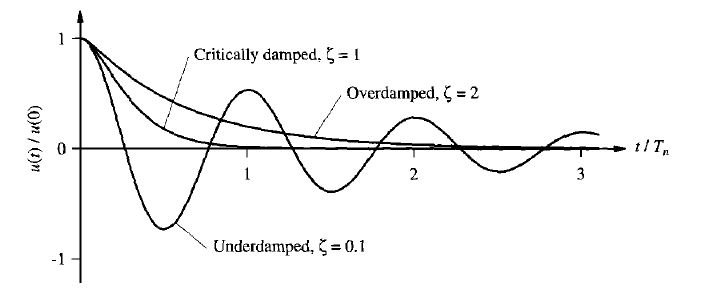
\includegraphics[width=\textwidth]{images/dampings.png}
\end{center}
Let us look at some examples:\\
\begin{align*}
    \lambda_1 & = -1 ,   & \lambda_2 & =-3    & \implies V_{C,h} & = A_1e^{-t}+A_2e^{-3t}            \\
    \lambda_1 & =-1 ,    & \lambda_2 & =-1    & \implies V_{C,h} & = A_1e^{-t}+A_2te^{-t}            \\
    \lambda_1 & = -1+2j, & \lambda_2 & =-1-2j & \implies V_{C,h} & = e^{-t}(A_1\sin(2t)+A_2\cos(2t))
\end{align*}
To find the particular solution one could substitute into the ODE and use the same method as previous circuits.\\
However, there are some shortcuts:
\begin{itemize}
    \item Constant input: the particular solution will be the input.
    \item Sinusoidal input: one can use SSS properties, and strategies like voltage
          division.
    \item Exponential input: no shortcut, use ODE.
\end{itemize}
\section{Non-Ideal Elements}
While we have been representing components as perfect inductors or capacitors,
but these do not exist. If that were the case, inductors or capacitors would be
used to store energy instead of batteries.\\ The non-ideal inductor, also known
as a parasitic inductor, has a representation that takes into account the
resistance of the inductor wire $R_s$, the capacitance between adjacent wires,
and finally, the Ferrite Core loss, $R_p$, which consists of Eddy current loss
and hysteresis loss.\\ Thus, a full representation of an inductor, in terms of
ideal elements, would be:
\begin{center}
    \begin{circuitikz}[american voltages, american currents]
        \draw (0,0)
        to[R, l=$R_s$] (0,1.5)
        to[L,l=$L$](0,3);
        \draw (0,3)
        to [short, -] (1,3)
        to [C, l^=$C_p$] (1,0)
        to [short, -] (2.5,0)
        to [R, l_=$R_p$] (2.5,3);
        \draw (0,0) to [short, -] (1,0);
        \draw (1,3) to [short, -] (2.5,3);
    \end{circuitikz}
\end{center}
However, for this course, the effect of the capacitor and the ferrite core loss are negligible, allowing us to ignore them. If the frequency were closer to the self resonant frequencies of the inductor, $C_p$ would become relevant.\\
The non-ideal capacitor has a wire inductance $L_s$, a wire resistance $R_s$, and a leakage, $R_p$, which allow us to model the capacitor as the following:
\begin{center}
    \begin{circuitikz}[american voltages, american currents]
        \draw (0,0)
        to[R, l=$R_s$] (0,1.5)
        to[L,l=$L_s$](0,3);
        \draw (0,0)
        to [short, -] (-1,0)
        to [C, l^=$C$] (-1,-1.5)
        to [short, -] (1,-1.5)
        to [R, l_=$R_p$] (1,0);
        \draw (0,0) to [short, -] (1,0);
    \end{circuitikz}
\end{center}
However, $L_s$ and $R_s$ are both negligible for this course's considerations, as they both have very small values.\\
These new representations of these components allow us to introduce a new topic, which is quality factor (Q).
\begin{align*}
    Q(j\omega)   & = \left\lvert\frac{\text{Reactance}}{\text{Resistance}}\right\rvert = \left\lvert\frac{\text{Im}(Z)}{\text{Re}(z)}\right\rvert \\
    \implies Q_L & = \frac{\omega L}{R_s},\quad Q_C = \omega R_p C
\end{align*}
By using non-ideal representations of these elements within circuits, such as the RLC circuit, circuits are modified to result in resonant properties distinct to those found with ideal components.\\
\begin{center}
    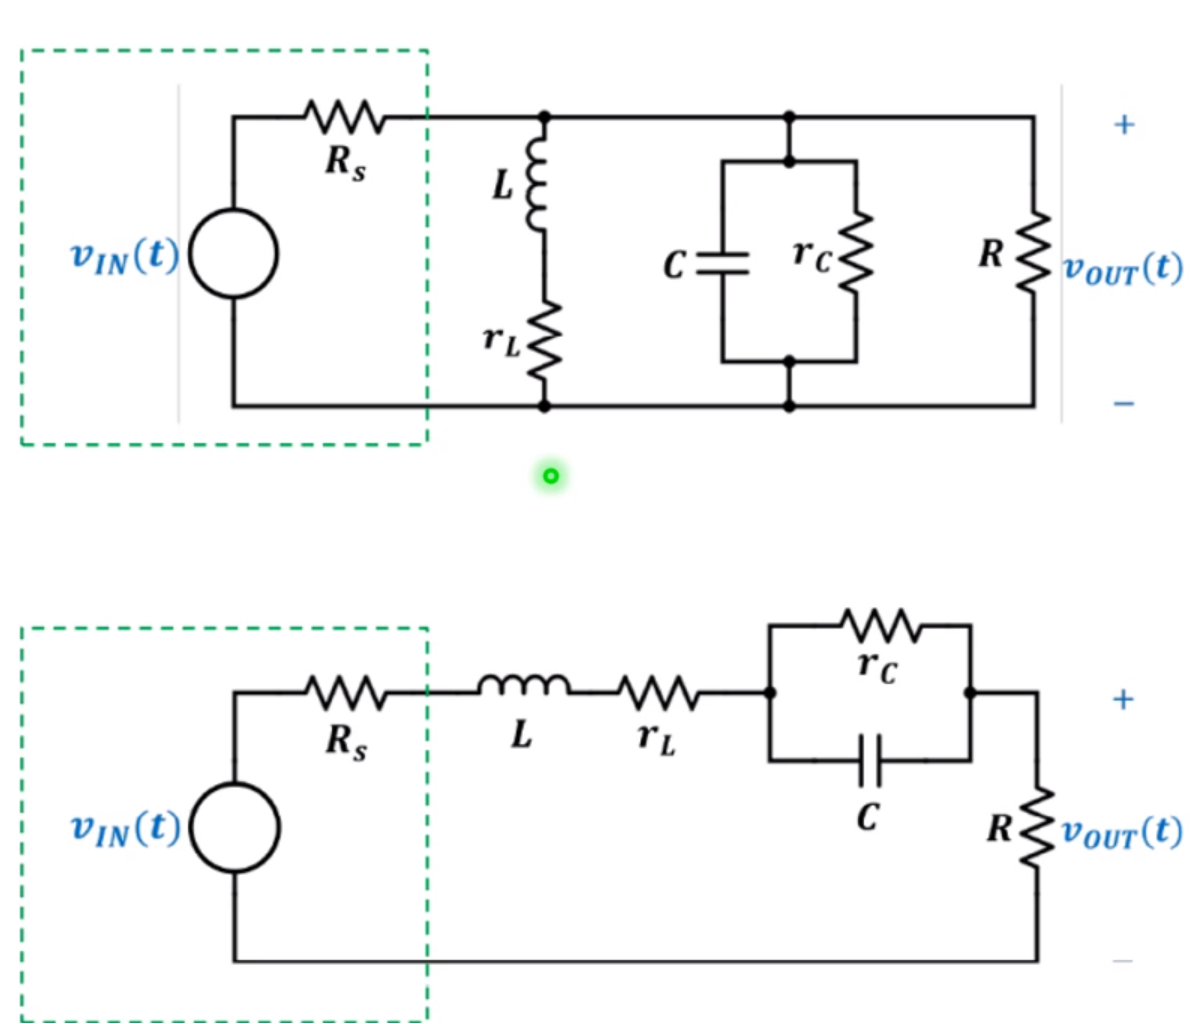
\includegraphics[width = 200px]{images/nonideal_rlc.png}
\end{center}
We will now learn to transform these configurations into more manageable and solvable configurations. \\
So, what we will try to do is to convert a series impedance and resistance configuration into a parallel one and vice-versa. That is, we want the parallel or series configuration with certain components to have the same impedance as the series or parallel configuration with the same components, but with different values.\\
\begin{align*}
    Z(j\omega)            & = R_s+jX_s                     & Y(j\omega)            & = G_p+jB_p                    \\
                          & = \frac{1}{G_p+jB_p}           &                       & =\frac{1}{R_s+jX_s}           \\
    G_p+jB_p              & = \frac{1}{R_s+jX_s}           & R_s+jX_s              & =\frac{1}{G_p+jB_p}           \\
                          & = \frac{R_s-jX_s}{R_s^2+X_s^2} &                       & =\frac{G_p-jB_p}{G_p^2+B_p^2} \\
    \implies G_p(j\omega) & = \frac{R_s}{R_s^2+X_s^2},     & \implies R_s(j\omega) & = \frac{G_p}{G_p^2+B_p^2},    \\
    B_p                   & = \frac{-X_s}{R_s^2+X_s^2}     & X_s(j\omega)          & = \frac{-B_p}{G_p^2+B_p^2}    \\
\end{align*}
With $Z$ being the impedance and $Y$ being the admittance.\\
Now, through a few operations, we van find the values of $L_p$ and $R_p$ that would be equivalent to what we want.\\
\begin{align*}
    L_p & =L_s\left(1+\left(\frac{R_s}{\omega L_s}\right)^2\right)=L_s\left(1+\frac{1}{Q_L^2}\right) \\
    R_p & =R_s\left(1+\left(\frac{\omega L_s}{R_s}\right)^2\right)=R_s(1+Q_L^2)                      \\
        & \text{At high Q:}                                                                          \\
    L_p & \approx L_s                                                                                \\
    R_p & \approx R_s Q_L^2
\end{align*}
This essentially means that at high Q, the inductor resembles an ideal inductor, as we would expect.\\
The same process can be conducted for capacitors:\\
\begin{align*}
    C_s & = C_p\left(1+\frac{1}{Q_c^2}\right) \\
    R_s & = \frac{R_p}{1+Q_c^2}               \\
        & \text{At high Q:}                   \\
    C_s & \approx C_p                         \\
    R_s & \approx \frac{R_p}{Q_c^2}
\end{align*}
These transformations should allow us to transform any non-ideal circuit into an equivalent circuit with ideal components, which we will be able to solve as shown in previous sections.\\
\textit{Note: unlike the original components, their transformations are frequency dependent.}\\
Another variable that may surge for non-ideal element questions is to find the self-resonant frequency of the circuit, which is $\omega_0=\frac{1}{\sqrt{LC_s}}$ or $\omega_0=\frac{1}{\sqrt{L_p C}}$ depending on the transformation.\\
This value can then be substituted into the equations for $Q$ related terms, allowing for simplification, and thus the value of the transformed resistor.
\section{Switched Circuits (Circuits with Switches)}
The current through an inductor is and will be continuous regardless of whether the voltage across it is continuous. This is because of the property of the current through an inductor that defines it as:
\begin{equation*}
    i_L(t)=\int_{t_0}^t v_L(\tau)d\tau
\end{equation*}
The same happens for capacitors and voltage.\\
This is relevant because it is often important to know how long it takes for an RL or RC circuit to go from one state to another.\\
We know that
\begin{equation*}
    x(t) = x(\infty) + (x(t_0^+)-x(\infty))e^{\frac{-(t-t_0)}{\tau}}
\end{equation*} 
What we want to discern is how long it will take for $x$ to go from the value $X_1$ to the value $X_2$.\\
\begin{align*}
    x(t_2) &= x(\infty) + (x(t_1)-x(\infty))e^{\frac{-(t_2-t_1)}{\tau}}\\
    x(t_2) - x(\infty) &= (x(t_1)-x(\infty))e^{\frac{-(t_2-t_1)}{\tau}}\\
    \frac{x(t_2)-x(\infty)}{x(t_1)-x(\infty)} &= e^{\frac{-(t_2-t_1)}{\tau}}\\
    \ln\left(\frac{x(t_2)-x(\infty)}{x(t_1)-x(\infty)}\right) &= \frac{-(t_2-t_1)}{\tau}\\
    \tau\ln\left(\frac{x(t_1)-x(\infty)}{x(t_2)-x(\infty)}\right) &= t_2-t_1\\
    \tau\ln\left(\frac{X_1-x(\infty)}{X_2-x(\infty)}\right) &= t_2-t_1
\end{align*} 
If this is used on circuits in specific situations, we can discern at what times a solution is relevant or valid.\\
\subsection{Important Functions and Function Transformations}
\textbf{Functions}\\
\begin{itemize}
    \item Unit Step Function:
    \begin{equation*}
        u(t) = \left\{
            \begin{array}{l}
                0 \quad t < 0 \\
                \text{undetermined} \quad t=0\\
                1 \quad t > 0 \\
            \end{array}
        \right.
    \end{equation*}
    \textit{Note: for most intents and purposes, $u(0)$ can be considered to be $1$ or irrelevant. However, non-continuous signals become undefined.\\~\\ Confused?\\ Different statements by different lecturers resulted in this statement.}
    \item Unit Function Shifted:
    \begin{equation*}
        u(t-t_0) = \left\{
            \begin{array}{l}
                0 \quad t < t_0 \\
                1 \quad t \geq t_0 \\
            \end{array}
        \right.
    \end{equation*}
    \item Rectangular Function:
    \begin{equation*}
        c(t) = u(t-t_1) - u(t-t_2) = \left\{
            \begin{array}{l}
                0 \quad t < t_1 \\
                1 \quad t_1 \leq t < t_2 \\
                0 \quad t \geq t_2\\
            \end{array}
        \right.
    \end{equation*}
    \item Dirac Function:
    \begin{equation*}
        \delta(x) = \left\{
            \begin{array}{l}
                +\infty \quad x = 0 \\
                0 \quad x \neq 0 \\
            \end{array}
        \right.
    \end{equation*}
    \begin{equation*}
        \int_{-\infty}^\infty \delta(\tau) d\tau = 1
    \end{equation*}
    \begin{equation*}
        \frac{du(t)}{dt} = \delta(t)
    \end{equation*}
\end{itemize}
\textbf{Transformations}
\begin{itemize}
\item If a function $f(t)$ changes to $f(t-b)$ it will shift to the right, and if it changes to $f(t+b)$ it will shift to the left.\\
\item If a function $f(t)$ changes to $f(at)$ with $|a| > 0$, it will expand along the x-axis, and if $|a| < 0$, it will contract. If $a$ is negative, it will be reflected about the x-axis.\\
\item If a function $f(t)$ changes to $cf(t)$, with $|c| > 1$, it will stretch along the y-axis, and if $|c| < 1$, it will contract. If $c$ is negative, it will be reflected about the y-axis.\\
\item If a function $f(t)$ changes to $f(t)+d$, with $d > 0$, it will shift up, and if $d < 0$, it will shift down.\\ Hello
\end{itemize}

\end{document}
